\subsection{Построение модели машинного обучения}
\label{sec:design:network}

Подробнее рассмотрим построение модели для определения жанра композиции. Для этого используют много подходов: метод опорных векторов, линейные регрессии, байесовы сети, нейронные сети и др. Остановимся на нейронных сетях, как на самом перспективном и передовом методе обработки данных.

Для того, чтобы повысить точность классификации, необходимо иметь достаточно высокий уровень абстракции. Поэтому небходимо воспользоваться методами глубого обучения. Глубокое обучение -- это часть более широкого семейства методов машинного обучения -- обучения представлениям, где векторы признаков располагаются сразу на множестве уровней. Эти признаки определяются автоматически и связывают друг с другом, формируя выходные данные. На каждом уровне представлены абстрактные признаки, основанные на признаках предыдущего уровня. Таким образом, чем глубже мы продвигаемся, тем выше уровень абстракции. В нейронных сетях множество слоев представляет собой множество уровней с векторами признаков, которые генерируют выходные данные.

Мы хотим, чтобы гибкость семейства функций росла при увеличении количества данных. В нейронных сетях мы изменяем количество скрытых элементов в зависимости от объема данных. Наши модели машинного обучения должны стать композиционными. Натуральные языки используют композиционность, чтобы представлять более сложные идеи. В глубоком обучении мы используем:
\begin{enumerate}
  \item распределенные представления;
  \item глубокую архитектуру.
\end{enumerate}

Давайте предположим, что данные поступают к нам не все сразу, а партиями. Партии могут поступать или параллельно, или последовательно. Параллельное поступление партий являет собой распределенное представление (обучение представлениям). Последовательное поступление данных похоже на обучение представлениям, но с несколькими уровнями. Композиционность дает нам возможность эффективного описания мира вокруг нас.

Нейронные сети разделяются на много типов:
\begin{enumerate}
  \item сети прямого распространения;
  \item нейронные сети Хопфилда;
  \item цепи Маркова;
  \item сверточные нейронные сети;
  \item рекуррентные нейронные сети;
  \item развертывающие нейронные сети;
  \item сети с долгой краткосрочной памятью и др.
\end{enumerate}

Для того, чтобы выбрать что-то, необходимо формализовать задачу. В исходном виде задачей является определение высокоуровневой характеристики музыкальной композиции, которая называется жанр. В более формальном виде задачу можно написать так: определить к какому классу принадлежит данная музыкальная композиция. Эта задача относится к задаче классификации.

В результате применения преобразования к композиции, мы получим матрицу большой размерности. Для того, чтобы классифицировать такую матрицу, необходимо извлечь из нее признаки. Для того, чтобы извлекать признаки из матрицы большого размера, стоит использовать сверточную нейронную сеть.

Для того, чтобы понять выбор данной архитектуры, надо понять как она работает. В отличие от обычной нейронной сети, слои CNN состоят из нейронов, расположенных в 3-х измерениях: ширине, высоте и глубине, то есть измерениях, которые формируют объем. Матрица предыдущего слоя сканируется небольшим окном и пропускается сквозь набор весов, а результат отображается на соответствующий нейрон текущего слоя. Таким образом, набор плоскостей представляет собой карты признаков, и каждая плоскость находит свои участки матрицы в любом месте предыдущего слоя. Входной слой предназначен лишь для подачи входной матрицы на следующий за ним слой и распределения входной матрицы по плоскостям. Следующий за входным слой называется свёрточным. Каждый нейрон в плоскости свёрточного слоя получает свои входы от некоторой области предыдущего слоя (локальное рецептивное поле), то есть входная матрица предыдущего слоя сканируется небольшим окном и пропускается сквозь набор весов, а результат отображается на соответствующий нейрон свёрточного слоя (см. рисунок \ref{sec:design:network:cnn_layers}). В итоге матрица будет преобразована в вектор признаков, который можно использовать для дальнейше классификации.

\begin{figure}[h]
\centering
	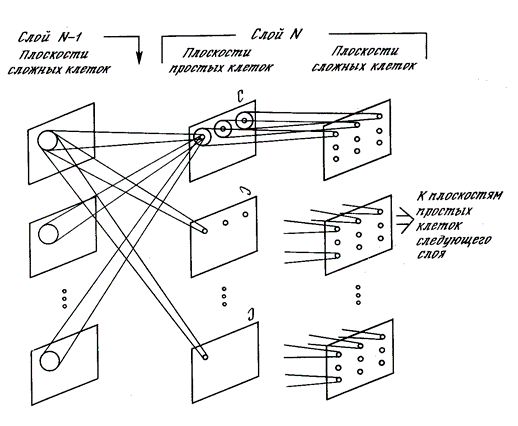
\includegraphics[scale=0.85]{cnn_principle.png}
	\caption{Принцип извлечения признаков сверточной нейронной сетью}
	\label{sec:design:network:cnn_layers}
\end{figure}

Для реализации необходимо разобраться из чего состоят слои сверточной нейронной сети. Слои сверточной нейронной сети состоят из:
\begin{enumerate}
  \item слой свертки, умножает значения фильтра на исходные значения элементов матрицы (поэлементное умножение), после чего все эти умножения суммируются;
  \item слой активации, применяет функцию активации к каждому \linebreak элементу;
  \item слой пулинга, выполняет операцию по понижающей дискретизации пространственных размеров (ширина и высота).
\end{enumerate}

Для того, чтобы оптимизировать обучение нейронной сети, необходимо выбрать функцию активации. Обычно в качестве функции активации используются сигмоидальные функции, например гиперболический тангенс. Использование гиперболического тангенса нецелесообразно, потому что на его вычисление уходит слишком много ресурсов. Поэтому стоит обратить внимание на другие функции активации. В нашем случае используется ELU (см. рисунок \ref{sec:design:network:elu}). ELU имеет отрицательные значения, что позволяет ей приближать средние активации к нулю. Ноль означает ускорение обучения, потому что они приближают градиент к естественному градиенту ELU.

\begin{figure}[h]
\centering
	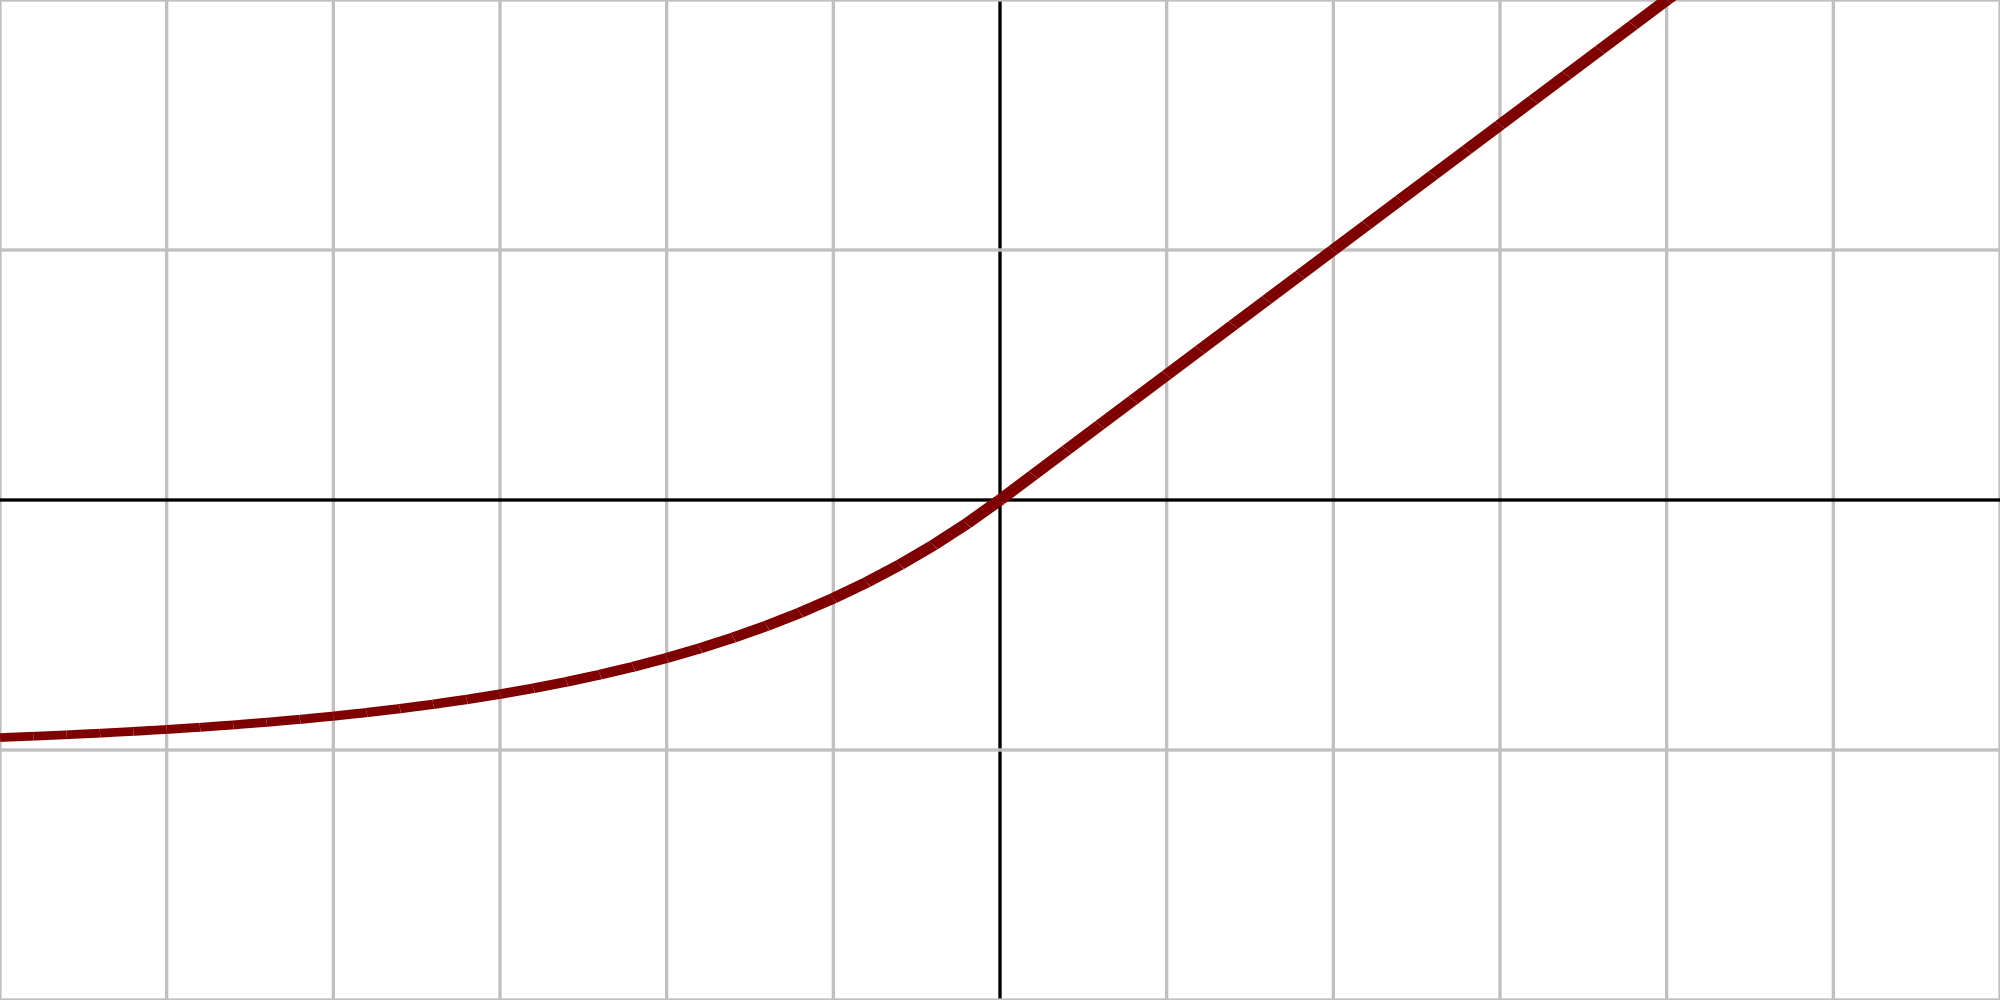
\includegraphics[scale=0.23]{elu.png}
	\caption{График функции активации ELU}
	\label{sec:design:network:elu}
\end{figure}

В дальнейшем нам необходимо классифицировать композицию по полученным признакам. Полученные признаки являются временной последовательностью, то есть их нельзя обрабатывать отдельно друг от друга. Для того, чтобы обрабатывать такие последовательности необходимо, чтобы на обработку текущих значений вляли текущие значения. Таким свойством обладает рекуррентная нейронная сеть.

Основное отличие рекурентных сетей (Recurrent Neural Network, RNN) от традиционных заключается в логике работы сети, при которой каждый нейрон взаимодействует сам с собой. На вход таким сетям как правило передаётся сигнал, являющийся некоторой последовательностью. Каждый элемент такой последовательности поочерёдно передаётся одним и тем же нейронам, которые своё же предсказание возвращают себе вместе со следующим её элементом, до тех пор пока последовательность не закончится. Такие сети, как правило, используются при работе с последовательной информацией -- в основном с текстами и аудио/видео-сигналами. Элементы рекурентной сети изображают как обычные нейроны с дополнительной циклической стрелкой, которая демонстрирует то, что кроме входного сигнала нейрон использует также своё дополнительное скрытое состояние. Если «развернуть» такое изображение, получится целая цепочка одинаковых нейронов, каждый из которых получает на вход свой элемент последовательности, выдаёт предсказание и передаёт его дальше по цепочке как своего рода ячейку памяти. Нужно понимать, что это абстракция, поскольку это один и тот же нейрон, который отрабатывает несколько раз подряд (см. рисунок \ref{sec:design:network:rnn_layer}).

\begin{figure}[h]
\centering
	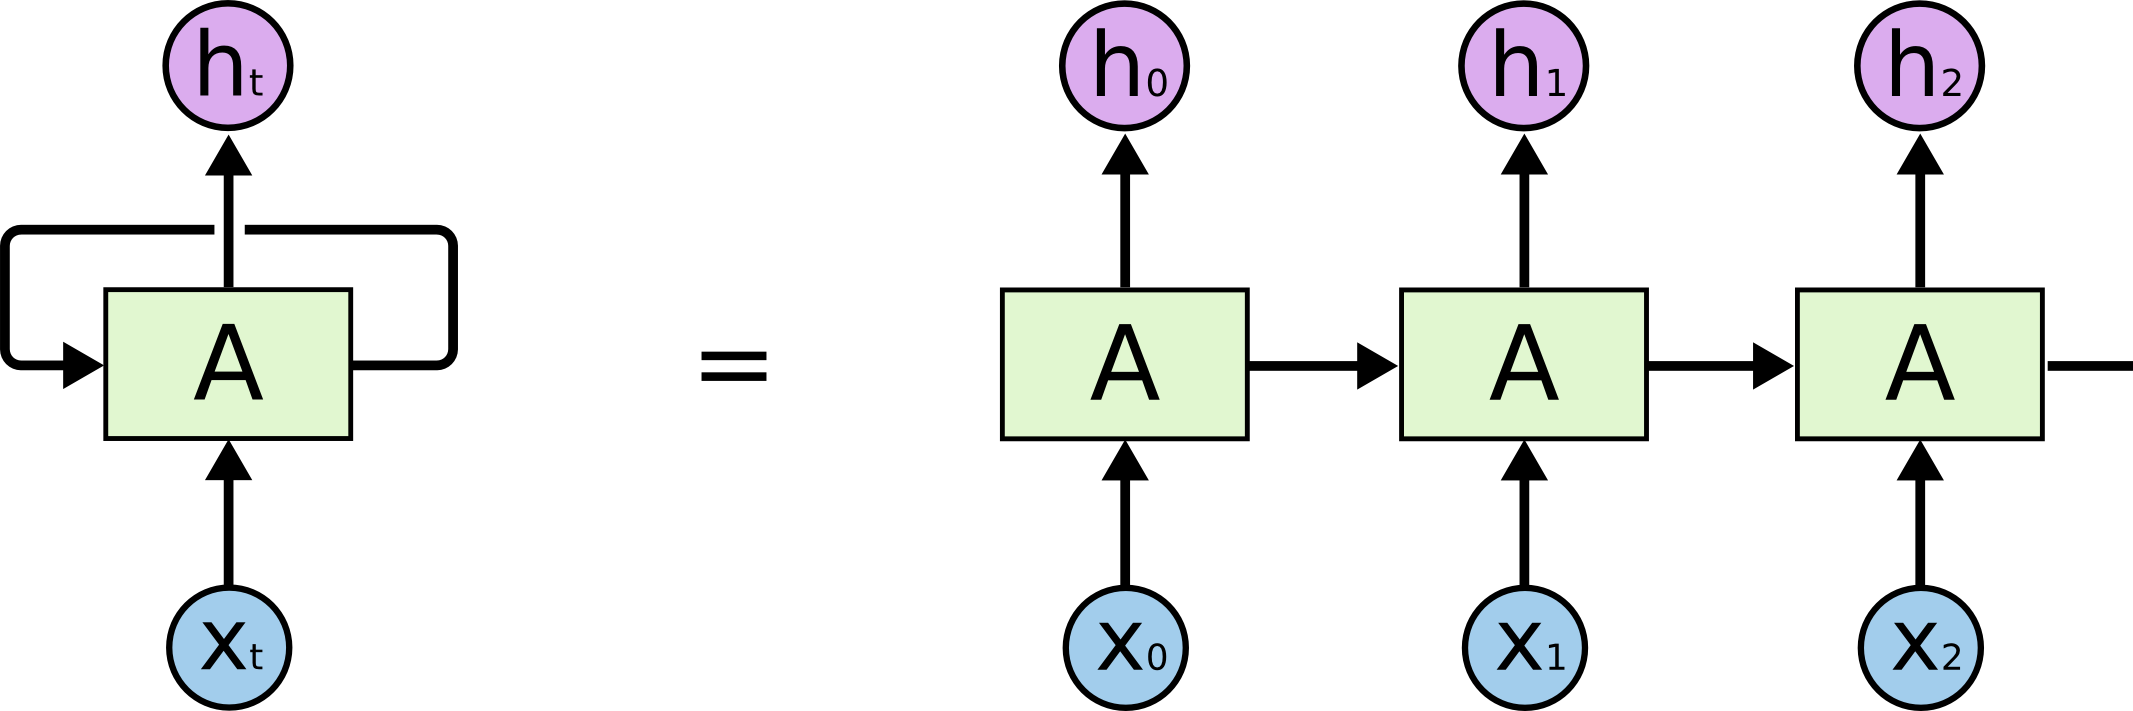
\includegraphics[scale=0.2]{rnn_layer.png}
	\caption{Принцип работы рекуррентной нейронной сети}
	\label{sec:design:network:rnn_layer}
\end{figure}

Моделирование памяти в нейронной сети подобным образом вводит новое измерение в описание процесса её работы — время. Пусть нейронная сеть получает на вход последовательность данных, например, текст пословно или слово побуквенно. Тогда каждый следующий элемент этой последовательности поступает на нейрон в новый условный момент времени. К этому моменту в нейроне уже есть накопленный с начала поступления информации опыт.

Итак, выбрав компоненты для построения архитектуры, необходимо определиться с составом нейронной сети. Выбрав слишком глубокую нейронную сеть, необходимо будет иметь большой объем данных, а так же большие вычислительные мощности. Так как объем данных, которыми мы обладаем не очень велик, а, главное, объем мощностей ограничен, то стоит ограничить количество слоев. Исследования показывают, что количество слоев, большее 6 требует значительных вычислительных мощностей для обучения. Меньшее количество слоев может привести к недостаточному уровню абстракции.

Для того, чтобы извлечение жанра было успешным, необходимо классифицировать композицию по признакам, которые имеют высокий уровень абстракции. Поэтому количество слоев сверточной нейронной сети должно превышать количество слоев рекуррентной нейронной сети. Так же использование совсем небольшого количества слоев для рекуррентной нейронной сети может повлиять отрицательно на классификацию временных признаков, которые были извлечены сверточной нейронной сеть, поэтому количество слоев рекуррентной нейронной сети должно быть не меньше 2.

Определившись с ограничениями, которые мы накладываем на нейронную сеть, можем определить её точный состав. Вход нейронной сети будет представлен четырьмя слоями сверточной нейронной сети, котороым будет поступать на вход матрица мел-спектральных коэффициентов. Слои реккурентной нейронной сети будут обрабатывать признаки, которые выделила сверточная нейронная сеть, и будет реализована в виде двух слоев.

Полученная нейронная сеть состоит из слоев: первые четыре -- сверточные, последующие два -- рекуррентные (см. рисунок \ref{sec:design:network:neuralnet}).

\begin{figure}[h]
\centering
	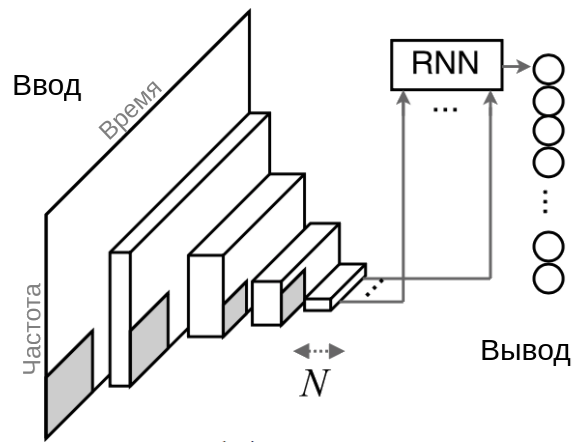
\includegraphics[scale=0.68]{diagrams.png}
	\caption{Полученная структура нейронной сети}
	\label{sec:design:network:neuralnet}
\end{figure}

Так же на скорость обучения влияет выбор оптимизатора. Стохастический градиентный спуск, который стал классическим для применения на нейронных сетях, слишком неоптимизирован. Другим алгоритмом оптимизации, присутствующим в сообществе нейронных сетей, является Adam. Adam можно рассматривать как обобщение AdaGrad (AdaGrad -- это Adam с определенным выбором параметров). Правило обновления для Adam определяется на основе оценки первого (среднего) и второго необработанного момента исторических градиентов (в рамках последнего временного окна через экспоненциальную скользящую среднюю). Эти статистические данные корректируются на каждой итерации (исправление необходимо из-за выбора инициализации).

Алгоритм оптимизации Adam:
\begin{enumerate}
  \item вычислить градиент в текущее время;
  \item обновить предварительную оценку первого момента;
  \item обновить смещенную оценку второго необработанного момента;
  \item вычислить оценку первого момента с исправлением смещения;
  \item вычислить скорректированную с учетом смещения оценку второго необработанного момента;
  \item обновить параметры.
\end{enumerate}

Так же мы можем столкнуться с проблемой переобучения. Она является очень важным подводным камнем глубокого обучения. Отрицательный эффект переобучения заметно проявляется на сетях, подобных той, что мы собираемся построить, а значит, необходимо найти способ защититься от этого явления прежде, чем мы пойдем дальше. К счастью, существует очень простой метод, который мы и применим.

Переобучение -- это излишне точное соответствие нейронной сети конкретному набору обучающих примеров, при котором сеть теряет способность к обобщению (см. рисунок \ref{sec:design:network:overfit}). Другими словами, наша модель могла выучить обучающее множество (вместе с шумом, который в нем присутствует), но она не смогла распознать скрытые процессы, которые это множество породили.

\begin{figure}[h]
\centering
	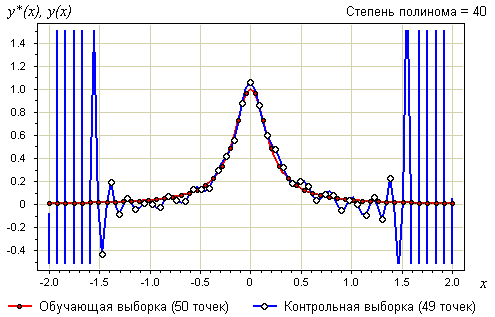
\includegraphics[scale=0.7]{overfit.png}
	\caption{Пример переобучения для полиномиальной функции}
	\label{sec:design:network:overfit}
\end{figure}

У глубоких сверточных нейронных сетей масса разнообразных параметров, особенно это касается полносвязных слоев. Переобучение может проявить себя в следующей форме: если у нас недостаточно обучающих примеров, маленькая группа нейронов может стать ответственной за большинство вычислений, а остальные нейроны станут избыточны; или наоборот, некоторые нейроны могут нанести ущерб производительности, при этом другие нейроны из их слоя не будут заниматься ничем, кроме исправления их ошибок.

Чтобы помочь нашей сети не утратить способности к обобщению в этих обстоятельствах, мы вводим приемы регуляризации: вместо сокращения количества параметров, мы накладываем ограничения на параметры модели во время обучения, не позволяя нейронам изучать шум обучающих данных. Dropout с параметром p за одну итерацию обучения проходит по всем нейронам определенного слоя и с вероятностью p полностью исключает их из сети на время итерации (см. рисунок \ref{sec:design:network:dropout}). Это заставит сеть обрабатывать ошибки и не полагаться на существование определенного нейрона (или группы нейронов), а полагаться на согласованное значение нейронов внутри одного слоя. Этот довольно простой метод позволяет эффективно бороться с проблемой переобучения, без необходимости использовать другие методы.

\begin{figure}[h]
\centering
	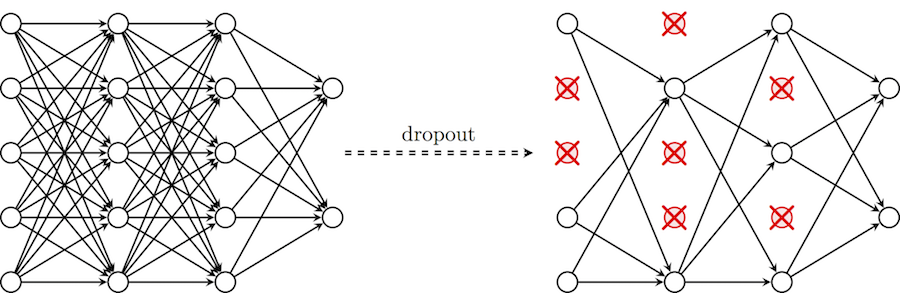
\includegraphics[scale=2.35]{dropout.png}
	\caption{Пример использования dropout}
	\label{sec:design:network:dropout}
\end{figure}
